\subsection{Transmisión}

Se desarrolló e implementó la comunicación entre el software SettDev y el PLC para transmitir los datos leídos desde el archivo. El PLC-Kaab de SEDPC se controla y comunica utilizando datagramas; éstos se envían por medio del protocolo UDP, y tienen un formato de trama específico, que es el que se muestra en la Figura \ref{fig:tramaPLC} obtenida del documento . La trama comienza con un encabezado (Header) que siempre contiene el valor 8A, seguido de algunas indicaciones para el PLC, como el proceso Fuente del que provienen los datos, el proceso de Destino, e indicaciones internas (Internal Indications). Luego, se indica un comando (Command), un subcomando (Subcommand), la indicación de algún Error producido, y la longitud $n$ de los datos por enviar (Largo). Los siguientes $n$ bytes contienen la información a enviar (Data). Por último, se calcula un Checksum como medio de comprobación de errores; si se produce algún error, el PLC no reproduce el datagrama enviado. Se utilizan identificadores con valores numéricos para indicar la Fuente o Destino (el proceso) que envía o recibe los datos, así como el comando y subcomando por ejecutar.

\begin{figure}[htb]
	\centering
	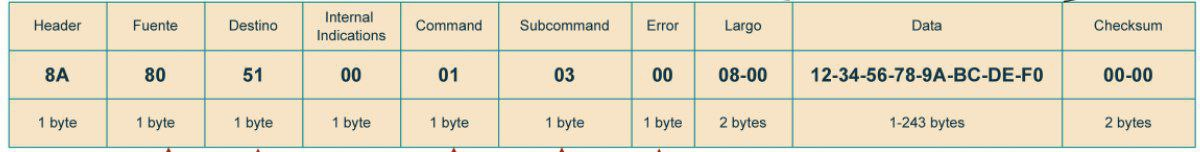
\includegraphics[scale=0.4]{tramaPLC.jpg}
	\caption{Formato de trama utilizado por el PLC-Kaab}
	\label{fig:tramaPLC}
\end{figure}

Para elaborar la trama, se tomó como referencia la que genera un módulo desarrollado por SEDPC en SettDev para controlar servomotores. En dicha interfaz, existen controles deslizantes que indican los ángulos enviados al PLC; los valores son transmitidos al dar clic a un botón ``Enviar''. El contenido de la trama generado por este módulo es el que se muestra en la Figura . Los campos Fuente y Destino contienen el valor 06, que hace referencia al proceso de Interfaz Gráfica de Usuario (el software SettDev, y el software contenido en el PLC); el comando 02 indica una escritura de datos en el PLC (en este caso, el nuevo ángulo); y el subcomando 06 indica una entrada de datos digitales (los datos contenidos en la trama). Como los errores se comprueban antes de enviar la trama, el campo Error siempre contiene el valor 00; el campo Largo indica que el tamaño del campo Data es de 19 bytes. En dicho campo, los datos se indican como sigue:

\begin{enumerate}
	\item Byte 1: Tipo de motor (el valor 1 identifica a los servomotores)
	\item Bytes 3-7: Nuevo ángulo en formato Little Endian
	\item Bytes 8-11: Pulso mínimo en formato Little Endian
	\item Bytes 12-15: Pulso máximo en formato Little Endian
	\item Bytes 16-19: Ángulo máximo en formato Little Endian
\end{enumerate}

En el formato Big Endian, que es el que comúnmente se utiliza para representar un valor digital, los bytes de izquierda a derecha se ordenan desde el más significativo hasta el menos significativo. En el formato Little Endian, este orden se invierte.